\documentclass[a4paper, 12pt]{bxjsarticle}
\usepackage{graphicx}
\usepackage{amsmath}
\usepackage{txfonts}
\usepackage{siunitx}
\usepackage{mathspec}
\setmainfont{IPAexMincho}
\setsansfont{IPAexGothic}
\XeTeXlinebreaklocale "ja"
\topmargin = 0mm
\pagestyle{empty}

\renewcommand{\thesubsection}{\arabic{subsection}.}
\renewcommand{\thesubsubsection}{(\alph{subsubsection})}

\begin {document}

\begin{samepage}
\begin{center}
    \begin{LARGE}
        {\huge 電磁気学 11/6 宿題} 
    \end{LARGE}
\end{center}

\vspace{-1em}
\subsection{点電荷 \(q\) を同心球殻の中心からずれた点に置く.導体内壁の電荷分布は不均一になる.では,外壁では均一か不均一か.}
\vspace{-1.5em}
\begin{figure}[h]
	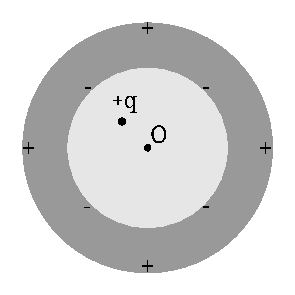
\includegraphics[scale=0.7]{drawing.pdf}
\end{figure}

\vspace{10em}

% p52, 問1.19
\subsection{地球を半径 \(6.4\times10^{6}\si{[m]}\) の導体球とみなして,その電気容量を計算せよ.}

\vspace{10em}
\end{samepage}
\newpage

% p52, 問1.20
\subsection{一辺 \(1.0\times10^{-1}\si{[m]}\) の正方形状金属板2枚を間隔 \(1.0\times10^{-3}\si{[m]}\) だけ離してつくった平行板コンデンサーの電気容量を計算せよ.}
\vspace{23em}

% p52, 問1.21
\subsection{p.48 図1.34(b) のように,電気容量 \(C_1,C_2,C_3,\ldots,C_N\)の \(N\) 個のコンデンサーを並列に接続したときの合成容量を求めよ.}

\newpage
% p50, 例題1.7.3をBaseにした問題
\subsection{p.51 図1.37のように,半径 \(a\),長さ \(l\) の円柱状導体と長さが同じで内半径 \(b\) の円筒状導体とを中心軸が一致するように配置して作ったコンデンサーの電気容量を求めよ.ただし導体間の間隔 \(b-a\) は導体の長さに比べて十分に小さく,電界は導体に挟まれた空間にのみ存在するとする.また,\(a=0.3\si{[mm]},\;b=2.0\si{[mm]}\) の円筒同軸ケーブルのキャパシタンスを求めよ.}
\end{document}
